\documentclass[12pt]{amsart}
\usepackage{amsthm}
\usepackage{graphicx}
\newcommand*\oct{\vcenter{\hbox{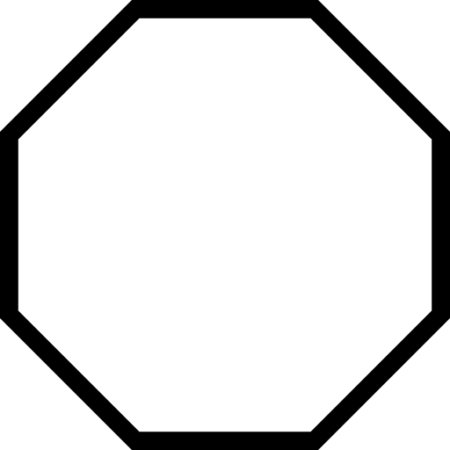
\includegraphics[width=.9em]{octagon.png}}}}
\newcommand{\F}{\mathcal{F}}
\newcommand{\Z}{\mathbb{Z}}

\newtheorem{theorem}{Theorem}
\newtheorem{lemma}{Lemma}
\newtheorem{corollary}{Corollary}

\theoremstyle{definition}
\newtheorem{definition}{Definition}

\title{Stopping Times}
\author{Robert Dougherty-Bliss and Charles Kenney}

\begin{document}
\maketitle

\section{Stopped binary strings}%
\label{sec:stopped_binary_strings}

\begin{definition}
    A \emph{binary string of length $n$} is a tuple $(x_1, x_2, \dots, x_n)$
    where each $x_k$ is $0$ or $1$. Such a string is said to be \emph{stopped}
    at index $k$ if every index of the tuple in $(k / 2, k]$ is zero. The
    \emph{stopping time} of a binary string is the smallest $k$ such that the
    string is stopped at index $k$, or $\infty$ if no such $k$ exists. Note
    that, except $1$ and $\infty$, every stopping time is even.
\end{definition}

We are primarily interested in binary strings of length $n$ which have stopping
time $n$. Indeed, let $g(n)$ be the number of such strings. Our first goal is
to show that $g(n)$ satifies the recurrence
\begin{align*}
    g(1) &= g(2) = g(4) = 1 \\
    g(4n) &= 2 g(4n - 2) \\
    g(4n + 2) &= 2 g(4n) - g(2n).
\end{align*}
This will identify the sequence $a(n) = g(2n)$ as the
\emph{Narayana--Zidek--Capell numbers}, A2083 in the OEIS, which begin
\begin{equation*}
    1, 1, 1, 2, 3, 6, 11, 22, 42, 84, 165, 330, 654, \dots
\end{equation*}
This recurrence was discovered thanks to the OEIS.

Our first definition discusses \emph{finite} binary strings, but it is more
convenient to work with \emph{infinite} binary strings which are nonzero in
only finitely many places. This is equivalent, and has the benefit that every
such infinite string has a finite stopping time when considered as a
sufficiently long, finite binary string.

\begin{definition}
    Let
    \begin{equation*}
        V = \bigoplus_{k=1}^\infty (\Z/2\Z)
    \end{equation*}
    be the direct sum of infinitely many copies of $\Z / 2\Z$. That is, the set
    of all infinite tuples $(x_1, x_2, x_3, \dots)$ where each $x_k$ is $0$ or
    $1$, and only finitely many are $1$. For each positive integer $k$, let
    $\oct_k$ be the set of elements of $V$ which are zero beyond position $k$
    and, when the first $k$ entries are regarded as a finite binary string,
    they have stopping time $k$. That is, $\oct_1 = \{0\} \subset V$,
    \begin{equation*}
        \oct_{2k} = \{v \in V : \forall j > k, v_j = 0, \text{ and } v \text{ has stopping time } 2k \}
    \end{equation*}
    and $\oct_{2k + 1} = \emptyset$ for every integer $k \geq 1$.
\end{definition}

It is clear that $g(n) = |\oct_n|$ for every positive integer $n$.

\begin{theorem}
    The sequence $g(n)$ satisfies the recurrence
    \begin{align*}
        g(1) &= g(2) = g(4) = 1 \\
        g(4n) &= 2 g(4n - 2) \\
        g(4n + 2) &= 2 g(4n) - g(2n).
    \end{align*}
\end{theorem}

% Todo
% Clean this up!
% Add details!
% (I [Robert] volunteer to do this.)
\begin{proof}
    Each nonzero element in $V$ has a final nonzero entry (a one). Let $e_0 \colon V
    \to V$ be a map which inserts a $0$ in the position of this final entry,
    shifting the previous final entry to the right one space. Similarly, let $e_1$ insert a $1$.
    Symbolically,
    \begin{equation*}
        e_0(b) =
            \begin{cases}
                0 \text{ if } b=0 \\
                (b_1, ..., b_j, 0, 1, 0,0,...) \text{ if } b = (b_1, ..., b_j, 1, 0, 0, ...)
            \end{cases}
    \end{equation*}
    and
    \begin{equation*}
        e_1(b) =
            \begin{cases}
                (1, 0, 0, \dots) \text{ if } b=0 \\
                (b_1, ..., b_j, 1, 1, 0,0,...) \text{ if } b = (b_1, ..., b_j, 1, 0, 0, ...).
            \end{cases}
    \end{equation*}
    Note that $e_0$ and $e_1$ are injective, $e_0(V) \cap e_1(V) = \emptyset,$
    and $e_0(V) \cup e_1(V) = V.$

    For any positive integer $k$,
    \begin{equation*}
        \oct_{2k + 2} \subseteq e_0(\oct_{2k}) \cup e_1(\oct_{2k}).
    \end{equation*}
    Indeed, the final nonzero entry of every string in $\oct_{2k + 2}$ occurs
    at position $k + 1$. Removing the immediately preceding entry produces a
    string in $\oct_{2k}$---$e_0$ and $e_1$ simply add the entry back.

    In the other direction, for $k \geq 2$ we have
    \begin{equation*}
        e_1(\oct_{2k}) \subseteq \oct_{2k + 2},
    \end{equation*}
    because inserting a $1$ into position $k$ will never decrease the stopping
    time. For \emph{odd} $k \geq 3$ we have
    \begin{equation*}
        e_0(\oct_{2k}) \subseteq \oct_{2k + 2},
    \end{equation*}
    because inserting a $0$ at position $k$ will only decrease the stopping
    time if the new stopping time \emph{is} $k$; this is impossible if $k$ is
    odd. This shows that
    \begin{equation*}
        \oct_{2k + 2} = e_0(\oct_{2k}) \cup e_1(\oct_{2k}),
    \end{equation*}
    and thus
    \begin{equation*}
        g(2k + 2) = 2 g(2k)
    \end{equation*}
    for $k$ odd.

    To handle the even case, let
    \begin{equation*}
        \oct_{2k}^1 = \{(b_1, ..., b_{2k}, 1, 0,0,...) \in V \text{ s.t. } (b_1,...,b_{2k},0,0,...) \in \oct_{2k}\}.
    \end{equation*}
    (Note that $|\oct_{2k}^1| = |\oct_{2k}| = g(2k)$.) Then
    \begin{equation*}
        e_0(\oct_{4k}) \subseteq \oct_{4k + 2} \cup \oct_{2k}^1.
    \end{equation*}
    This implies
    \begin{equation*}
        \oct_{4k + 2} \cup \oct_{2k}^1 = e_0(\oct_{4k}) \cup e_1(\oct_{4k}).
    \end{equation*}
    (That the left contains the right is clear given the preceding inclusion.
    For the other direction, note $\oct_{2k}^1 \subseteq
    e_0(\oct_{4k})$, since if $(b_1, ..., b_{2k}, 0,0,...) \in \oct_{2k}$ then
    $(b_1, ..., b_{2k-1},1,0,0,...)$ has stopping time precisely $4k$.) Therefore
    \begin{equation*}
        g(4k + 2) + |\oct_{2k}^1| = 2 g(4k),
    \end{equation*}
    or
    \begin{equation*}
        g(4k + 2) = 2 g(4k) - g(2k).
    \end{equation*}
    This establishes the recurrence.
\end{proof}

\section{Stopped reals in the unit interval}
\label{sec:stopped_points_in_the_unit_interval}

Every element of the unit interval $[0, 1]$ can be regarded, via its binary
expansion, as an infinite binary string, i.e., an element of $\Z / 2 Z \times
\Z / 2Z \times \cdots$. This differs from the set $V$ of the previous section
by allowing potentially infinitely many nonzero entries. For example, the real
\begin{equation*}
    (0.1010101010101\dots)_2 = \frac{2}{3}
\end{equation*}
is perfectly well-defined, but not as a member of $\bigoplus_{k = 1}^\infty (\Z
/ 2 \Z)$. In this way, it makes since to discuss stopped \emph{reals},
considering each real as an infinite binary string. (We shall interchangably
refer to reals as both strings and numbers.) Our focus now becomes
\emph{topological} as we examine the \emph{set} of stopped reals in the unit
interval.

\begin{definition}
    Let $S_k$ be the set of reals in $[0, 1]$ which have stopping time $k$ when
    regarded as an infinite binary string. Membership in this set is determined
    by examining only the first $k$ bits of a binary expansion, so $S_k$ is
    measureable. Let $S = \cup_{k \geq 1} S_k$ be the set of all stopped reals
    in $[0, 1]$, which is measurable since the $S_k$ are.
\end{definition}

Let us get a feel for what the sets $S_k$ ``look like.'' First, observe that
every element of $S_k$ consists of a binary string which has stopping time $k$
followed by \emph{any} binary string at all. Thus, each string with stopping
time $k$ determines an interval of length $2^{-k}$ included in $S_k$, and the
disjoint union of these intervals is \emph{all} of $S_k$. In this way, we can
compute the following sets:
\begin{align*}
    S_1 &= [0, 1/2) \\
    S_2 &= [1/2, 3/4) \\
    S_4 &= [3/4, 13/16) \\
    S_6 &= [7/8, 57/64) \\
    S_8 = [13/16, 209/256) &\cup [15/16, 241/256).
\end{align*}

[Insert the stopping time plot somewhere around here.]

This simple description of $S_k$ gives us a nice expression for the measure of
$S$.

\begin{theorem}
    Let $\beta_2$ be the measure of $S$. Then
    \begin{equation*}
        \beta_2 = \sum_{k \geq 1} \frac{g(k)}{2^k} = \frac{1}{2} + \sum_{k \geq 1} \frac{g(2k)}{4^k}
        \approx 0.841657913173647.
    \end{equation*}
\end{theorem}

\begin{proof}
    The measure of $S_k$ is $g(k) / 2^k$, where $g(k)$ is the number of binary
    strings of length $k$ with stopping time $k$. Since $S$ is the pairwise
    disjoint union of the $S_k$, the ``exact'' result follows immediately.
\end{proof}

In the previous section we established that the sequence $a(n) = g(2n)$ is
A2083 in the OEIS. It is known that $a(n) = O(2^n)$, so the above series
converges very quickly. Using the recurrence of the previous section to
generate the first hundred terms of $g(2k)$ it is easy to approximate the sum
and provide rigorous lower bounds. To get more rigorous upper bounds, first
note $g(2n) / 2^n$ is monotonically decreasing. This implies that the error of
using
\begin{equation*}
    \frac{1}{2} + \sum_{1 \leq k < n} \frac{g(2k)}{4^k}
\end{equation*}
as an approximation to the measure of $S$ is
\begin{equation*}
    \sum_{k \geq n} \frac{g(2k)}{4^k}
        \leq \frac{g(2n)}{2^n} \sum_{k \geq n} \frac{1}{2^k}
        = \frac{2g(2n)}{4^n}.
\end{equation*}
For example, using the first $99$ terms ($n = 100$) will give an error of no
more than
\begin{equation*}
    \frac{22284668265087}{158456325028528675187087900672}
    \approx 0.1406360286 \times 10^{-15}.
\end{equation*}

The constant $\beta_2$ seems new. We conjecture that it is irrational, and even
transcendental. In fact, the only thing we know about it is that it is a value
of the ordinary generating function of $g(n)$.

\begin{definition}
    Let
    \begin{equation*}
        G(z) = \sum_{k \geq 0} g(k) z^k = z + \sum_{k \geq 1} g(2k) z^{2k}
    \end{equation*}
    be the ordinary generating function of $g(n)$, and
    \begin{equation*}
        A(z) = \sum_{k \geq 1} g(2k) z^k
    \end{equation*}
    the ordinary generating function of $g(2k)$. Note that $G(z) = z + A(z^2)$.
\end{definition}

\begin{lemma}
    The generating function $A(z)$ is analytic on a disk of radius $1 / 2$
    centered at the origin and satisfies
    \begin{equation*}
        A(z) = \frac{z(1 - A(z^2))}{1 - 2z}.
    \end{equation*}
\end{lemma}

\begin{proof}
    The equation is a routine computation using the recurrence for $g(2n)$ proved in
    the previous section. For convenience, let $a(n) = g(2n)$. Then:
    \begin{align*}
        \sum_{k \geq 1} a(k) z^k
            &= \sum_{k \geq 1} a(2k) z^{2k} + \sum_{k \geq 0} a(2k + 1) z^{2k + 1} \\
            &= \sum_{k \geq 1} 2 a(2k - 2) z^{2k} + a(1) z + \sum_{k \geq 1} (2a(2k) - a(k)) z^{2k + 1} \\
            &= 2 z \sum_{k \geq 0} a(2k + 1) z^{2k + 1} + 2 z \sum_{k \geq 1} a(2k) z^{2k} - z A(z^2) + z \\
            &= 2z A(z) + z(1 - A(z^2)).
    \end{align*}
    Solving this for $A(z)$ yields the result. It is well-known that $a(n) =
    O(2^n)$, so $A(z)$ converges everywhere that $\sum_{k \geq 0} (2z)^k = (1 -
    2z)^{-1}$ does, which is at least a disk of radius $1/2$.
\end{proof}

It is clear that
\begin{equation*}
    \beta_2 = G(1/2) =\frac{1}{2} + A(1/4).
\end{equation*}
But again, this is very little information. We suspect that neither $A(z)$ nor
$G(z)$ are algebraic.

Our choice of notation for $\beta_2$---including a subscript $2$---is quite
intentional. Everything that we have done with binary sequences generalizes
almost directly to arbitrary bases. Take the definitions we gave before and
replace any occurrence of ``$1$'' with ``nonzero entry.'' Almost everything
that we have said carries over, except that the recurrence for $g(n)$ is
slightly different. We will now give these definitions in order to define an
infinite family $\{\beta_n\}$ of constants.

\begin{definition}
    For any integer $b \geq 2$, say that a finite ``$b$-ary'' tuple $(x_1,
    \dots, x_n)$ with $x_k \in \{0, 1, \dots, b - 1\}$ is \emph{stopped} at an
    index $k$ provided that every index in $(k / 2, k]$ is zero. The
    \emph{stopping time} of such a string is the smallest $k$ such that the
    string is stopped at $k$, or $\infty$ if no such $k$ exists. The stopping
    time of an infinite tuple is the stopping time of its shortest stopped
    prefix, or $\infty$ if no such prefix exists.
\end{definition}

\begin{definition}
    For any integer $b \geq 2$, let $g_b(n)$ be the number of $b$-ary strings
    of length $n$ with stopping time $n$.
\end{definition}

The same argument used in Theorem~1 (defining, now, $e_0$, $e_1$, and so on up
to $e_{b - 1}$) will establish the following result.

\begin{theorem}
\end{theorem}

\end{document}
